\subsubsection{A Three-Dimensional Model}

As well as models constructed from primitive two-dimensional shapes, we can extend these models into three dimensions. Some solutions are simple expansions of these primitives into their three-dimensional counter parts, but others are more intricate. M. Yamamoto et al used Computer Aided Design to develop a model constructed of conical cylinders and cuboids\cite{cadmodel}. Another example of this is shown in Figure~\ref{fig:3dmodelajd} where a range of three-dimensional shapes are mapped to a human figure by J. Deutscher et al.

\begin{figure}[H]
    \centering
    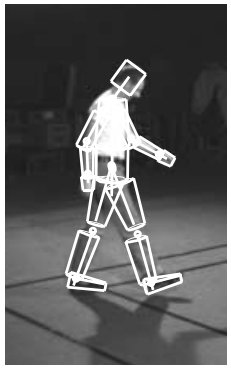
\includegraphics[height=6cm]{background/images/3dpolygon}

	\caption{A model constructed of three-dimensional primitive shapes\cite{stickfigure}}
	\label{fig:3dmodelajd}
\end{figure}

Some have used more advanced techniques to construct a customised model to be used to track a known person. C. Wu et al performed a three-dimensional scan of the subjects to generate a textured model of each person to be tracked\cite{capturystereopaper}. Several others have used similar techniques, creating a more `life like' model of a human. This has advantages in being able to fit the subject more accurately, but requires an additional step to create the model of a new subject prior to tracking them. Figure~\ref{fig:3dtexturedmodel} shows an example of a model generated in this way and mapped to a frame of video.

\begin{figure}[H]
    \centering
    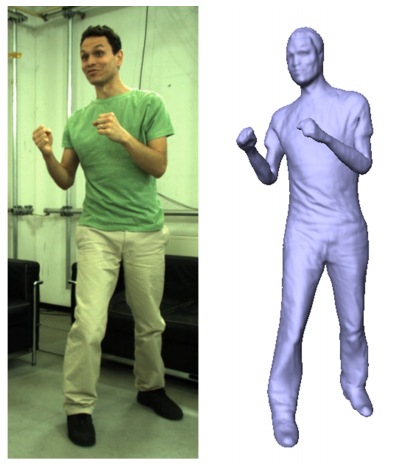
\includegraphics[height=6cm]{background/images/3dtexture}

	\caption{A more advanced model, specific to an individual subject\cite{capturystereopaper}}
	\label{fig:3dtexturedmodel}
\end{figure}